%%
%% This is file `sample-workshop.tex', adopted from
%% `sample-sigconf.tex',
%% generated with the docstrip utility.
%%
%% The original source files were:
%%
%% samples.dtx  (with options: `sigconf')
%% 
%% IMPORTANT NOTICE:
%% 
%% For the copyright see the source file.
%% 
%% Any modified versions of this file must be renamed
%% with new filenames distinct from sample-sigconf.tex.
%% 
%% For distribution of the original source see the terms
%% for copying and modification in the file samples.dtx.
%% 
%% This generated file may be distributed as long as the
%% original source files, as listed above, are part of the
%% same distribution. (The sources need not necessarily be
%% in the same archive or directory.)
%%
%% The first command in your LaTeX source must be the \documentclass command.
\documentclass[sigconf]{acmart}
\usepackage{hologo}
\usepackage{caption}
\usepackage{subcaption}
%%
%% \BibTeX command to typeset BibTeX logo in the docs
 % \AtBeginDocument{%
 %  \providecommand\BibTeX{{B\kern-.05em\hbox{$\m@th$\csname S@\f@size\endcsname\fontsize\sf@size\z@\math@fontsfalse\selectfont I\kern-.025emB}\kern-.08em\-\TeX}}% {%
  % % \normalfont B\kern-0.5em~{\scshape i\kern-0.25em~ b}\kern-0.8em\quad\TeX}}


%% Rights management information.  This information is sent to you
%% when you complete the rights form.  These commands have SAMPLE
%% values in them; it is your responsibility as an author to replace
%% the commands and values with those provided to you when you
%% complete the rights form.
\setcopyright{none}%acmcopyright}
\copyrightyear{}%2018}
\acmYear{}%2018}
\acmDOI{}%10.1145/1122445.1122456}

%% These commands are for a PROCEEDINGS abstract or paper.
\acmConference[Learning from Data Project Report]{Learning from Data Project Report}{December 31, 2019}{Shenzhen, China}
% \acmBooktitle{TBSI-WODS '19, Student Research Competition,
%   December 17--19, 2019, Shenzhen, China}
 \acmPrice{}%15.00}
 \acmISBN{}%978-1-4503-XXXX-X/18/06}
\settopmatter{printacmref=false}

%%
%% Submission ID.
%% Use this when submitting an article to a sponsored event. You'll
%% receive a unique submission ID from the organizers
%% of the event, and this ID should be used as the parameter to this command.
%%\acmSubmissionID{123-A56-BU3}

%%
%% The majority of ACM publications use numbered citations and
%% references.  The command \citestyle{authoryear} switches to the
%% "author year" style.
%%
%% If you are preparing content for an event
%% sponsored by ACM SIGGRAPH, you must use the "author year" style of
%% citations and references.
%% Uncommenting
%% the next command will enable that style.
%%\citestyle{acmauthoryear}

% page limit
% https://stackoverflow.com/questions/2720534/force-a-maximum-number-of-pages-in-latex
\makeatletter
\newcounter{pagecount}
\newcommand{\limitpages}[1]{
    \setcounter{pagecount}{0}%
    \gdef\maxpages{#1}%
    \ifx\latex@outputpage\@undefined\relax%
        \global\let\latex@outputpage\@outputpage%
    \fi%
    \gdef\@outputpage{%
        \addtocounter{pagecount}{1}%
        \ifnum\value{pagecount}>\maxpages\relax%
            % Do not output the page
        \else%
            \latex@outputpage%
        \fi%
    }%
}
\makeatother

%%
%% end of the preamble, start of the body of the document source.
\begin{document}
\limitpages{10}

%%
%% The "title" command has an optional parameter,
%% allowing the author to define a "short title" to be used in page headers.
\title{Multi-Zone Taxi Order Demand Prediction}

\author{Pengshun Li}
\affiliation{%
  \institution{lps19@mails.tsinghua.edu.cn}}

\author{Chenxi Cheng}
\affiliation{%
  \institution{ccx19@mails.tsinghua.edu.cn}}

\author{Chenyu Tian}
\affiliation{%
  \institution{tiancy19@mails.tsinghua.edu.cn}}


\begin{abstract}
  Travel order demand prediction is of great importance for the improvement of intelligent transportation system to city-scale and personalized services. An accurate short-term travel demand prediction model in both spatial and temporal relations can help the city pre-allocate resources and facilitate city-scale travel operation management in megacity. 
  To address problems like this, in this project, we propose a multi-zone order demand prediction model to predict short-term order demand in different zones at city-scale. Two-step methodology was developed including order zone division and multi-zone order prediction. For the zone division step, the K-Means++ spatial clustering algorithm was used. For the prediction step, six methods, LWLR, GA-BP Neural Network, SVR, average fusion-based method, weighted fusion-based method and kNN fusion based method are compared.
  These models were performed and validated on a real-world taxi order demand data from 3-month consecutive collection in Shenzhen, China.
\end{abstract}

\maketitle

\section{Introduction}
Traffic has always been an important factor in the city management and operation which impacts the daily life of millions of dwellers. Nowadays, with the demand for upgrading the intelligent transportation system to provide more smart and personalized services, travel demand is needed to be calculated in real-time for city-scale system operation because most of the traffic inefficiency are caused by imbalanced travel demand and supply. The better we can predict travel order demand, the better can help the city pre-allocate resources and facilitate city-scale travel operation management in megacity. For example, for sharing service, it can help facilitate the schedule of sharing vehicle fleet in advanced to reduce the costly cruise expense; for taxi operation management, it can reduce the imbalance between taxi supply and demand in some areas. To conclude, predicting travel demand can not only help individuals to save time and get more benefits but also helps to improve the efficiency of the urban traffic system.

Based on that, an accurate short-term multi-zone travel demand prediction model is needed. In our project, a two-step methodology was developed including order zone division and multi-zone order prediction. In the first step, the input to our algorithm is the geographic coordinates of taxi orders. We then use the K-means++ to output clustered zones. In the second step, the input to our algorithm is the historical taxi order demand data. We then use multiple methods (LWLR, GA-BP Neural Network, SVR, average fusion-based method, weighted fusion-based method, kNN fusion based method) to predict the taxi demand in these zones. 
\section{Related Work}
Actually, there is no exact same but only similar tasks in the literatures. There have been many prediction studies for traffic scenarios, including traffic volume, taxi demand, traffic flow volume and these studies propose some prediction methods. 
To predict traffic, time series analysis methods are the most popular models. Representatively, autoregressive integrated moving average (ARIMA) are well-known time series forecasting models by its short-term prediction performance\cite{li2012prediction}. More recently, machine learning methods have been frequently used to predict future traffic data, which attempt to identify historical data that are similar to the prediction instant, including neural networks (NN), support vector regression (SVR), random forest (RF), k-Nearest Neighbours (kNN) and so on. Habtemichael and Cetin\cite{habtemichael2016short} proposed an enhanced k-Nearest Neighbours algorithm for short-term traffic forecasting and it indicated that the proposed method can provide promising results. Nikravesh\cite{nikravesh2016mobile} compared some machine learning methods in terms of predicting traffic data, and the result showed that SVM performed better in predicting the multidimensionality of network traffic data. But individual prediction methods do not provide good enough predictive performance.

In order to further reduce prediction error, in recent years, some researchers research methods to combine prediction models to improve prediction accuracy\cite{guo2017influence}. Qiu proposed an integrated precipitation-correction model to use fusion method with four prediction models to predict freeway traffic flow\cite{qiu2016integrated}. Vlahogianni\cite{vlahogianni2015optimization} combined three different prediction models to propose a surrogate model for freeway traffic speed prediction. And these studies verified that the fusion-based prediction model could improve prediction accuracy. 

According to the literature, it can be found that many studies on travel order demand prediction methods 
concerned more on temporal change. In order to have better prediction performance and be adapted to city-scale development, 
some researches consider the spatial effect on predictive performance. For example, some researches do research on travel 
order demand prediction for hot spot analysis or grids. Li\cite{li2012prediction} analyzed the spatial-temporal variation of passengers
in a hot spot. Ke\cite{ke2017short} used a state-of-the-art deep learning approach called the fusion convolutional long short-term 
memory network to predict passenger demand under on-demand ride services for 77 grids in Hangzhou, China by analyzing spatial-temporal
characteristics. However, currently, most researches focus on the hot spot or evenly divided grid zones, there is no study about multi-zone
prediction analysis considering order spatial distribution and overall performance for zone prediction as well, which is the biggest uniqueness of our project. 


\section{Dataset and Features}
\subsection{Data Description}
The data in this study come from the taxi order data consecutively collected from August 10 to October 23, 2015 in Shenzhen, China. The order data include information such as order ID, order time, order longitude and latitude as shown in \textit{Table 1}.
\begin{table}
  \caption{Data Description}
  \label{tab:freq}
  \begin{tabular}{ccl}
    \toprule
    Attribute&Description&Example\\
    \midrule
    number\_id&car license id& $\ast \ast 0115H$ \\
    on\_time&boarding time& 2015-08-03T04:47:52.000Z \\
    on\_GPS&boarding GPS time& 2015-08-03T04:47:56.000Z \\
    on\_difference&time difference& 4 \\
    on\_longitude&boarding longitude& 113.79980944 \\
    on\_latitude&boarding latitude& 22.69250807 \\
    off\_time&drop-off time& 2015-08-03T05:05:40.000Z \\
    off\_GPS&drop-off GPS time& 2015-08-03T05:05:36.000Z \\
  \bottomrule
\end{tabular}
\end{table}
The content of this study is to take order prediction in the urban area to Shenzhen Airport for example, so it does not consider order demand outside the city. The latitude and long range of Shenzhen is $22^{\circ}$45’ $\sim$ $22^{\circ}$82’ North latitude, and $113^{\circ}$71' $\sim$ $114^{\circ}$37' East longitude which is the area of the study zone. Then the data in the above range is selected. Furthermore, as we predict travel order demand to the airport, so it is necessary to extract order data which the order destination points are at Shenzhen Airport. The extraction results are visualized as shown in Fig.1. (blue points are order origin points, and the orange points are order destination points at Shenzhen Airport).

This project takes the taxi order demand to Shenzhen Airport on Tuesday as an example to predict the travel order demand to Shenzhen Airport in different zones within 60 minutes on this day. We select the GPS data of all Shenzhen taxi orders from September 1, 2015 to September 31, 2015 and calculate the order demand to the airport within time interval of 60 minutes, and then do the correlation analysis of the factors that influence travel demand to the airport by taxi. With 60 minutes as time interval, a day can be equally divided into 24 periods.

The data of all working day attributes from August 10, 2015 to October 18, 2015 were selected as a training dataset, and the data of all working day attributes from October 19, 2015 to October 23, 2015 were sorted out as a testing dataset. And cross-validation is used to select parameters.
\subsection{feature Selection}
Do the correlation analysis of the factors that influence travel demand to the airport by taxi
to better select input features as shown in \textit{Figure 1}.
% correlation_analysis2
\begin{figure}[ht]
  \begin{subfigure}{.5\textwidth}
    \centering
    % include first image
    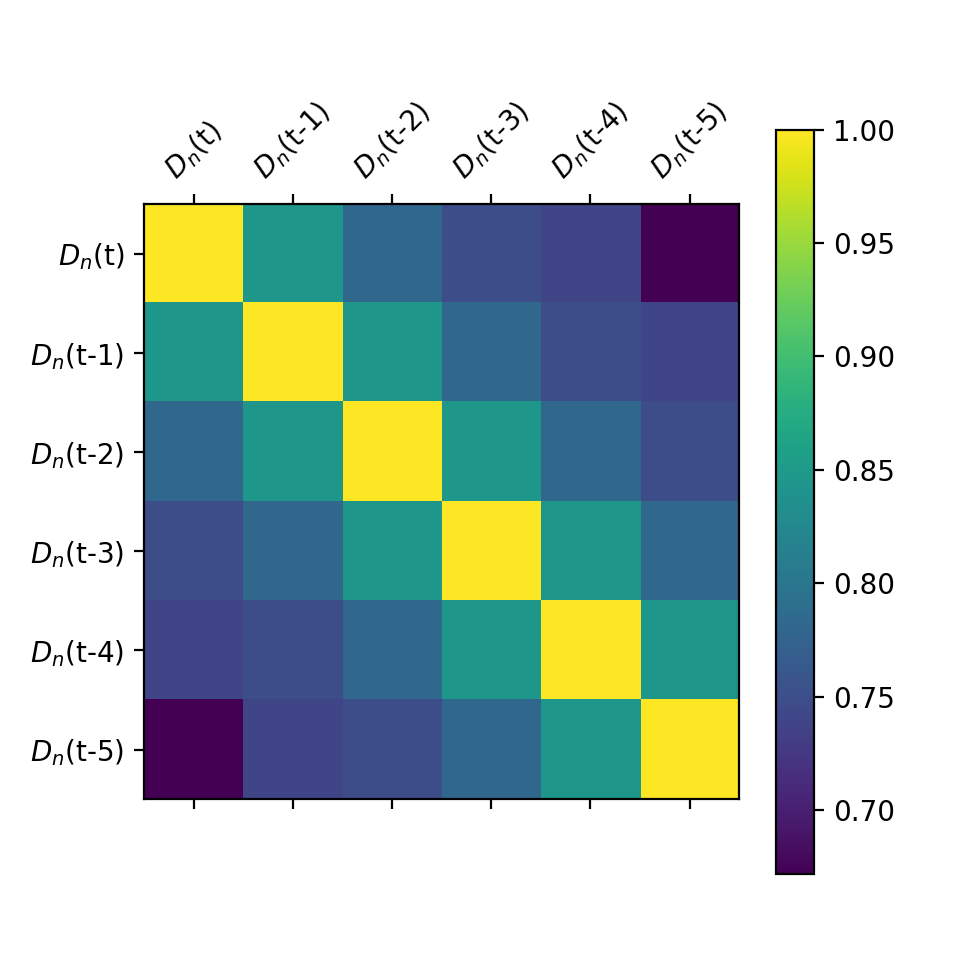
\includegraphics[width=.8\linewidth]{correlation_analysis1}  
    % \label{fig:sub-first}
  \end{subfigure}
  \begin{subfigure}{.5\textwidth}
    \centering
    % include second image
    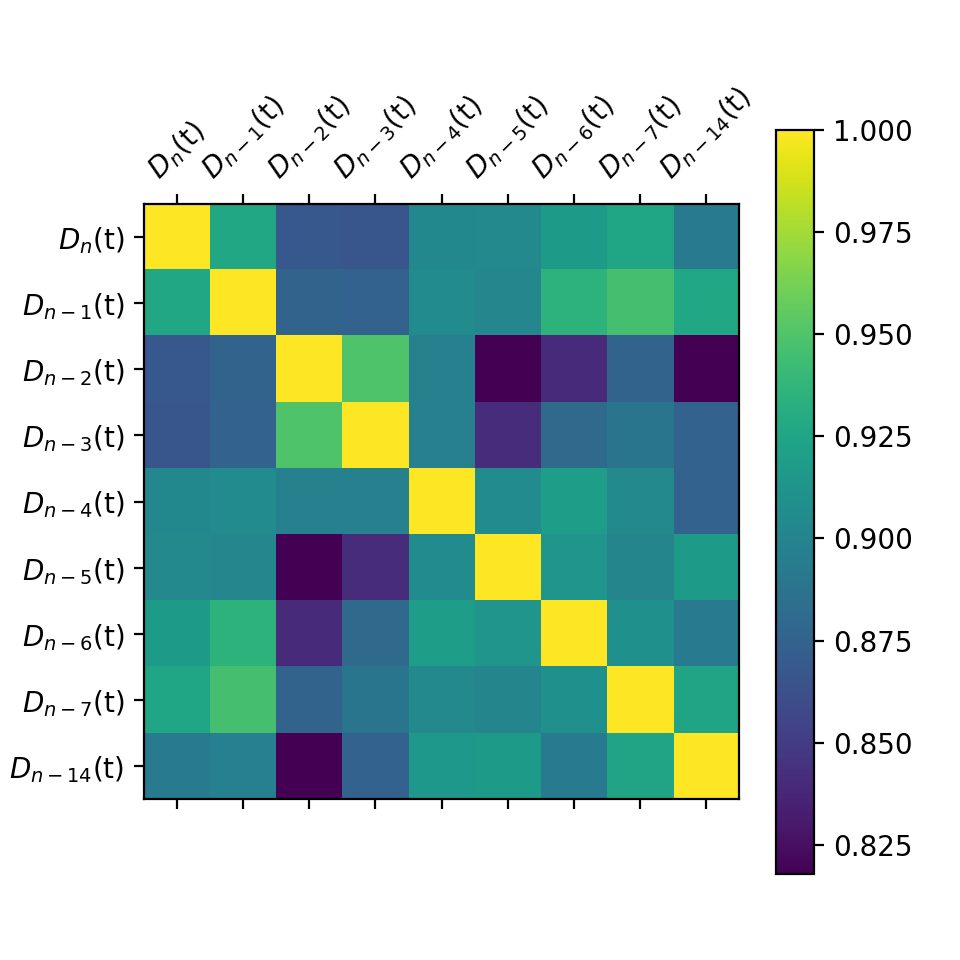
\includegraphics[width=.8\linewidth]{correlation_analysis2}  
    % \label{fig:sub-second}
  \end{subfigure}
  \caption{Correlation analysis}
  % \label{fig:fig}
  \end{figure}
Here define $D_{n}(t)$ is the taxi travel demand to the airport during period $[t, t+1)$ of day $n$.
Based on the correlation matrix, on a certain working day, the demand of the current period $D_{n}(t)$ has a higher correlation with $D_{n}(t-1), D_{n}(t-2)$, which are selected as features. 
And for the same time period in different days, the correlations of the same time in different working days are quite different. Therefore, when predicting order demand, we can choose $D_{n-1}(t)$, $D_{n-4}(t)$, $D_{n-5}(t)$, $D_{n-6}(t)$, $D_{n-7}(t)$ as input variables.

\section{Methods}
\subsection{Zone Division}
We have learnt the K\-means algorithm in the class. K\-Means++ algorithm is an algorithm that optimizes the initialization centroids based on K-Means algorithm. 
But for this algorithm, the number of clusters need to be prefined. It may have some problems when have no
knowledge about the number. 
Thus, we refered to BWP (Between-Within Proportion) index to select optimal number of clusters.
The basic idea is to find small intra-class distance as well as big inter-class distance.
The larger the average BWP value is, the better the clustering effect of the data set is, and among them, the number of clusters corresponding to the maximum value is the optimal clustering number.
Using this index to calculate the value of k clusters in the range of $[k_{min},k_{max}]$, the optimal number of clusters can be obtained.

\subsection{Order Prediction}
In this part, six prediction models are trained and tested.
  \subsubsection{Locally Weighted Linear Regression}
  Locally Weighted Linear Regression is a nonparametric learning algorithm\cite{cleveland1979robust}.
  When predicting new sample values, the training samples need to be trained to update the value of the parameter for each prediction.
  The values of new samples need to be predicted based on the training data sample set, so the values of the model parameter in each iteration are uncertain.
  The model allocates weights to each point near the point to be predicted based on the principle that the closer the distance, the greater the weight.
  Then the ordinary linear regression is performed using the minimization criterion of mean square error to predict the predicted value of the point to be predicted. The wavelength parameter k affects the accuracy of the model, a reasonable value of k is conducive to the improvement of prediction accuracy. In the optimisation process, the trial and error method is used, so the optimal wavelength parameter can be set.
  \subsubsection{Genetic Algorithm Back Propagation}
  BP Neural Network is a multi-layer feedforward neural network based on error back propagation\cite{chauvin2013backpropagation}.
  The basic idea is to use the network mean square error as the objective function. Based on the gradient descent strategy,
  the parameters are adjusted in the negative gradient direction of the target to minimize the error mean square error between the expected output value and the true value. BP Neural Network model has the advantage of approximating non-linear function with arbitrary precision, but it also has the disadvantage of being easily trapped in local optimum. 
  While GA-BP can use genetic algorithm to make the solution jump out of the local optimum and approximate the global optimum to optimize the weights and thresholds of the BP neural network, so the prediction results can be more accurate.
  Cross-validation for the selection of parameters is used in this study. After minimizing the Mean Absolute Percentage Error in the process of optimization, the number of hidden layer could be determined.
  \subsubsection{Support Vector Regression}
  Support Vector Regression (SVR) is a popular machine learning method that emerged at the end of the 20th century.
  It is mainly used for classification and prediction, and has good generalization ability.
  It is proposed by the world-renowned scholar Vapnik\cite{vapnik2013nature}. The SVR continuously
  adjusts the parameters by training the samples to derive a model that minimizes the sum
  of the deviations between the predicted and true values of all training samples.
  By inputting the predicted input vector into the model, the prediction can be made.
  In this project, a Radial Basis Function (RBF) is used as the kernel function because it is shown to be more suitable for traffic prediction under different conditions\cite{guo2017influence}.
  After optimising, the capacity values C of SVR can be determined and the insensitive loss function is used in this research.
  \subsubsection{Average Fusion based Method}
  Average fusion-based method (or blending) gives the average of the prediction results of each individual predictor. Given a set of predictors $\hat{y}^i$, we seek to compute final prediction , given by
  \begin{equation}
    \hat{y}=\frac{1}{m}\left(\hat{y}^{1}+\hat{y}^{2}+\ldots+\hat{y}^{m}\right)
  \end{equation}
  \subsubsection{Weighted fusion based method}
  In this method, or called bagging, weights of different predictors are not same. Weighted hybrid method is written as:
  \begin{equation}
    \begin{array}{c}{\hat{y}=\alpha_{1} \hat{y}^{1}+\alpha_{2} \hat{y}^{2}+\ldots+\alpha_{m} \hat{y}^{m}=\sum_{i} \alpha_{i} \hat{y}^{i}} \\ {\alpha_{1}+\alpha_{2}+\ldots+\alpha_{m}=1}\end{array}
  \end{equation}
  where $\alpha_{i}$ is the weight of i-th predictor. Weights are calculated using training dataset. In this study, the weights are calculated by the inverse of Mean Absolute Percentage Error (MAPE).
  \subsubsection{kNN Fusion based Method}
  The kNN fusion based method is highly unstructured and does not require any pre-determined model specification. The basic idea of kNN fusion-based method is, under the circumstance of current traffic state, to search the nearest neighbours to this state in the training used historical dataset to compute the prediction errors of the nearest neighbour set, estimate weights of each predictor, and combine the final predicted outputs of each individual predictor based on these weights\cite{guo2018predictor}.
  There are two steps in the kNN fusion-based method.
  
  The first step is to find the nearest neighbours, which are the historical observations that are most similar to the current observation. Euclidean distance is used in this study to determine the distance between the current input feature vector and historical observations. k is the number of historical observations with the nearest distances to the input feature vector.
  The second step is to calculate weights of each predictor.
  For each vector $x$, the predicted value ${\hat{y}=\sum_{i} \alpha_{i} \hat{y}^{i}}$, which has the same form as weighted fusion based method.
  The main difference between them is the weighted used in kNN fusion-based method is dynamically updated in every step calculated by the inverse of MAPE on the selected nearest neighbor dataset.

\subsection{Prediction Accuracy Indicator}
In order to better compare and analyze actual prediction performance and effect of different prediction models, predictors need to be evaluated and analyzed. In this work, some prediction performance evaluation indicators are adopted, including Mean Absolute Error (MAE), Mean Absolute Percentage Error (MAPE), Root Mean Square Error (RMSE).
And we then propose multi-zone weighted indicators based on MAE, MAPE, RMSE to evaluate the overall prediction performance of these prediction models in all the zones, including multi-zone weighted MAE indicator (MZW-MAE), multi-zone weighted MAPE indictor (MZW-MAE), multi-zone weighted RMSE indictor (MZW-RMSE) which are tailored for this task:
\begin{equation}
  \begin{array}{c}{\textit{MZW-MAE}=\sum_{k} \frac{O_{k}}{O} MAE_{k}} \\ {\textit{MZW-MAPE}=\sum_{k} \frac{O_{k}}{O} MAPE_{k}} \\ {\textit{MZW-RMSE}=\sum_{k} \frac{O_{k}}{O} RMSE_{k}}\end{array}
\end{equation}
where $O$ is the number of order demand in all zones, $O_k$ is the number of order demand in zone $k$, ${MAE}_k$, ${MAPE}_k$, ${RMSE}_k$ are the prediction accuracy indicators for zone $k$.

At the same time, a new evaluation rule is defined. When the predicted value of more than half of the predictors in a certain period is less than 7, the time period does not enter the evaluation range, because if the predicted demand is lower than 7, it indicates that during this period few people need travel in taxi, thus the prediction for this period is useless.

\section{Experiments}
\subsection{Zone Divison}
The order demand to Shenzhen Airport differ between working days and non-working days, and passenger travel demands have a strong regularity in working days. Therefore, this section only divides the working days’ order zone as case study.
The range of the value of $k$ is limited to [2, 30] by experience and actual conditions. After calling the K-Means++ algorithm, the BWP value curve is obtained as \textit{Figure 2}.
\begin{figure}[h]
  \centering
  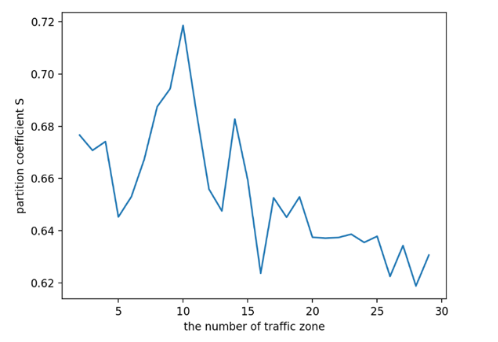
\includegraphics[width=1\linewidth]{figure1}
  \caption{Curve of BWP value with k value}
\end{figure}
When the value of $k$ is 10, the value of BWP is the largest. Hence, the number of order area in this task is determined to be 10. \textit{Figure 3} is a clustering result graph, and after visualizing the clustering data.
\begin{figure}[h]
  \centering
  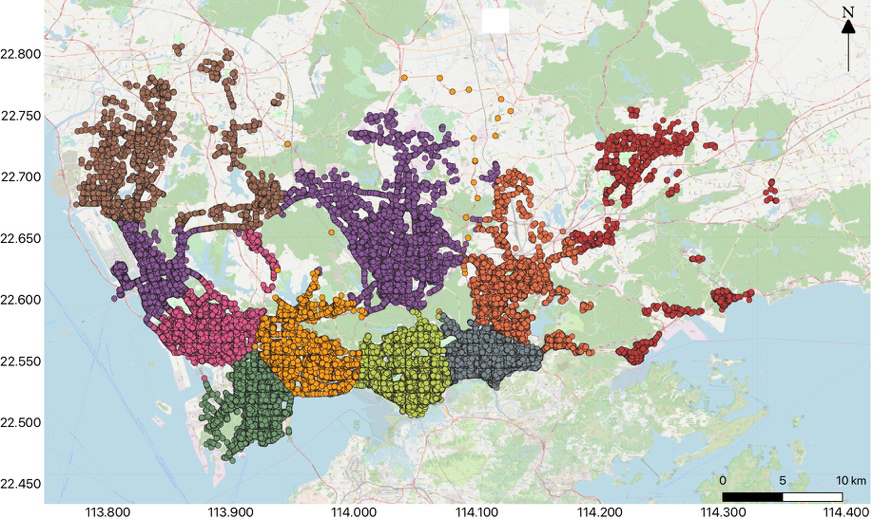
\includegraphics[width=1\linewidth]{figure2}
  \caption{The visualization of clustering result}
\end{figure}
Then, we connect the boundary points and fine-tune them based on the principle that one zone does not cross the main road as soon as possible, because when a driver cruises to find the passengers, they do not need to cross the main road, which could save cruise time. The order zones are fine-tuned and numbered, and Fig.3 is obtained.
\begin{figure}[h]
  \centering
  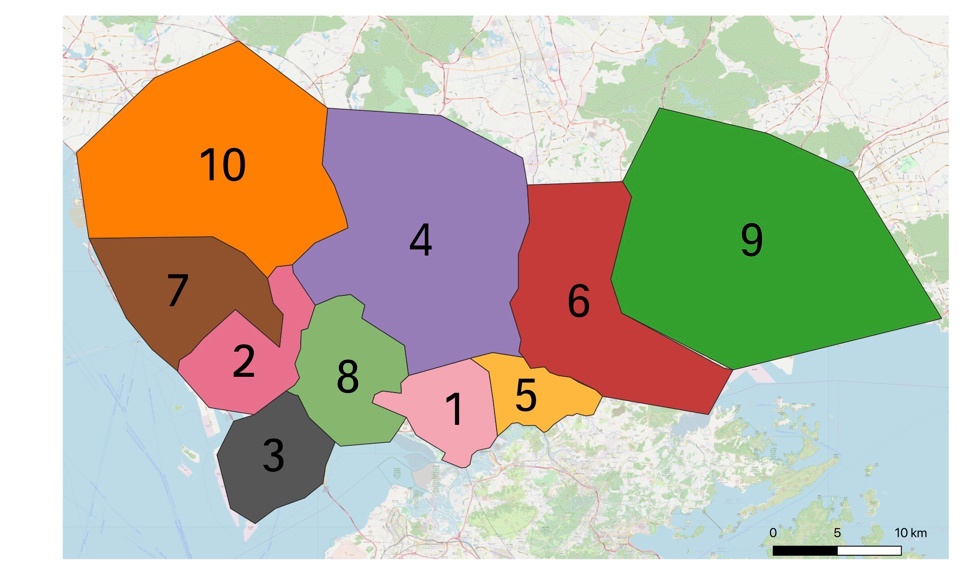
\includegraphics[width=1\linewidth]{figure3}
  \caption{Order zones are adjusted and numbered}
\end{figure}



\subsection{Order Prediction}
It can be seen from \textit{Figure5} that the prediction curves
of the various prediction models are generally consistent
with the overall trend of the actual observations
(Instead of showing all the figures of 10 zones, here just show prediction in zone 1).
During the peak period (5:00-8:00), each individual
prediction model including LWLR, GABP and SVR has
a good performance with no obvious deviation. Despite
this, they have different performances in other time
periods, which sometimes have good performance and sometimes
have poor performance. Fusion based prediction models
including average fusion based method, weighted fusion
based method and kNN fusion based method combine the
advantages of three individual prediction models and
slightly perform better than individual prediction models
in other periods (i.e. 10:11:00 in zone 1). 
\begin{figure}[h]
  \centering
  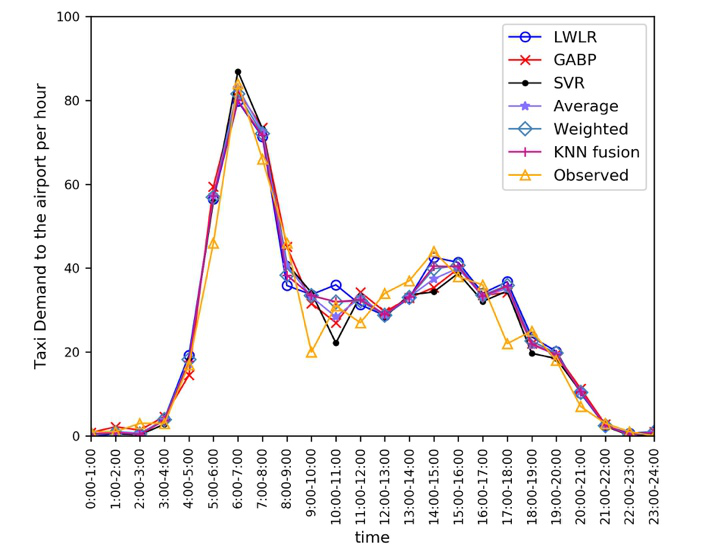
\includegraphics[width=1\linewidth]{zone1}
  \caption{Predicted and observed results in zone 1}
\end{figure}
To better compare and analyse the prediction performances of different prediction models, Mean Absolute Error (MAE), Mean Absolute Percentage Error (MAPE), Root Mean Square Error (RMSE) are adopted. Furthermore, multi-zone weighted MAE indicator (MZW-MAE), multi-zone weighted MAPE indictor (MZW-MAE), multi-zone weighted RMSE indictor (MZW-RMSE) are adopted to evaluate the overall prediction performance of these prediction models in all the zones.
\begin{figure*}
  \begin{subfigure}{.5\textwidth}
    \centering
    % include first image
    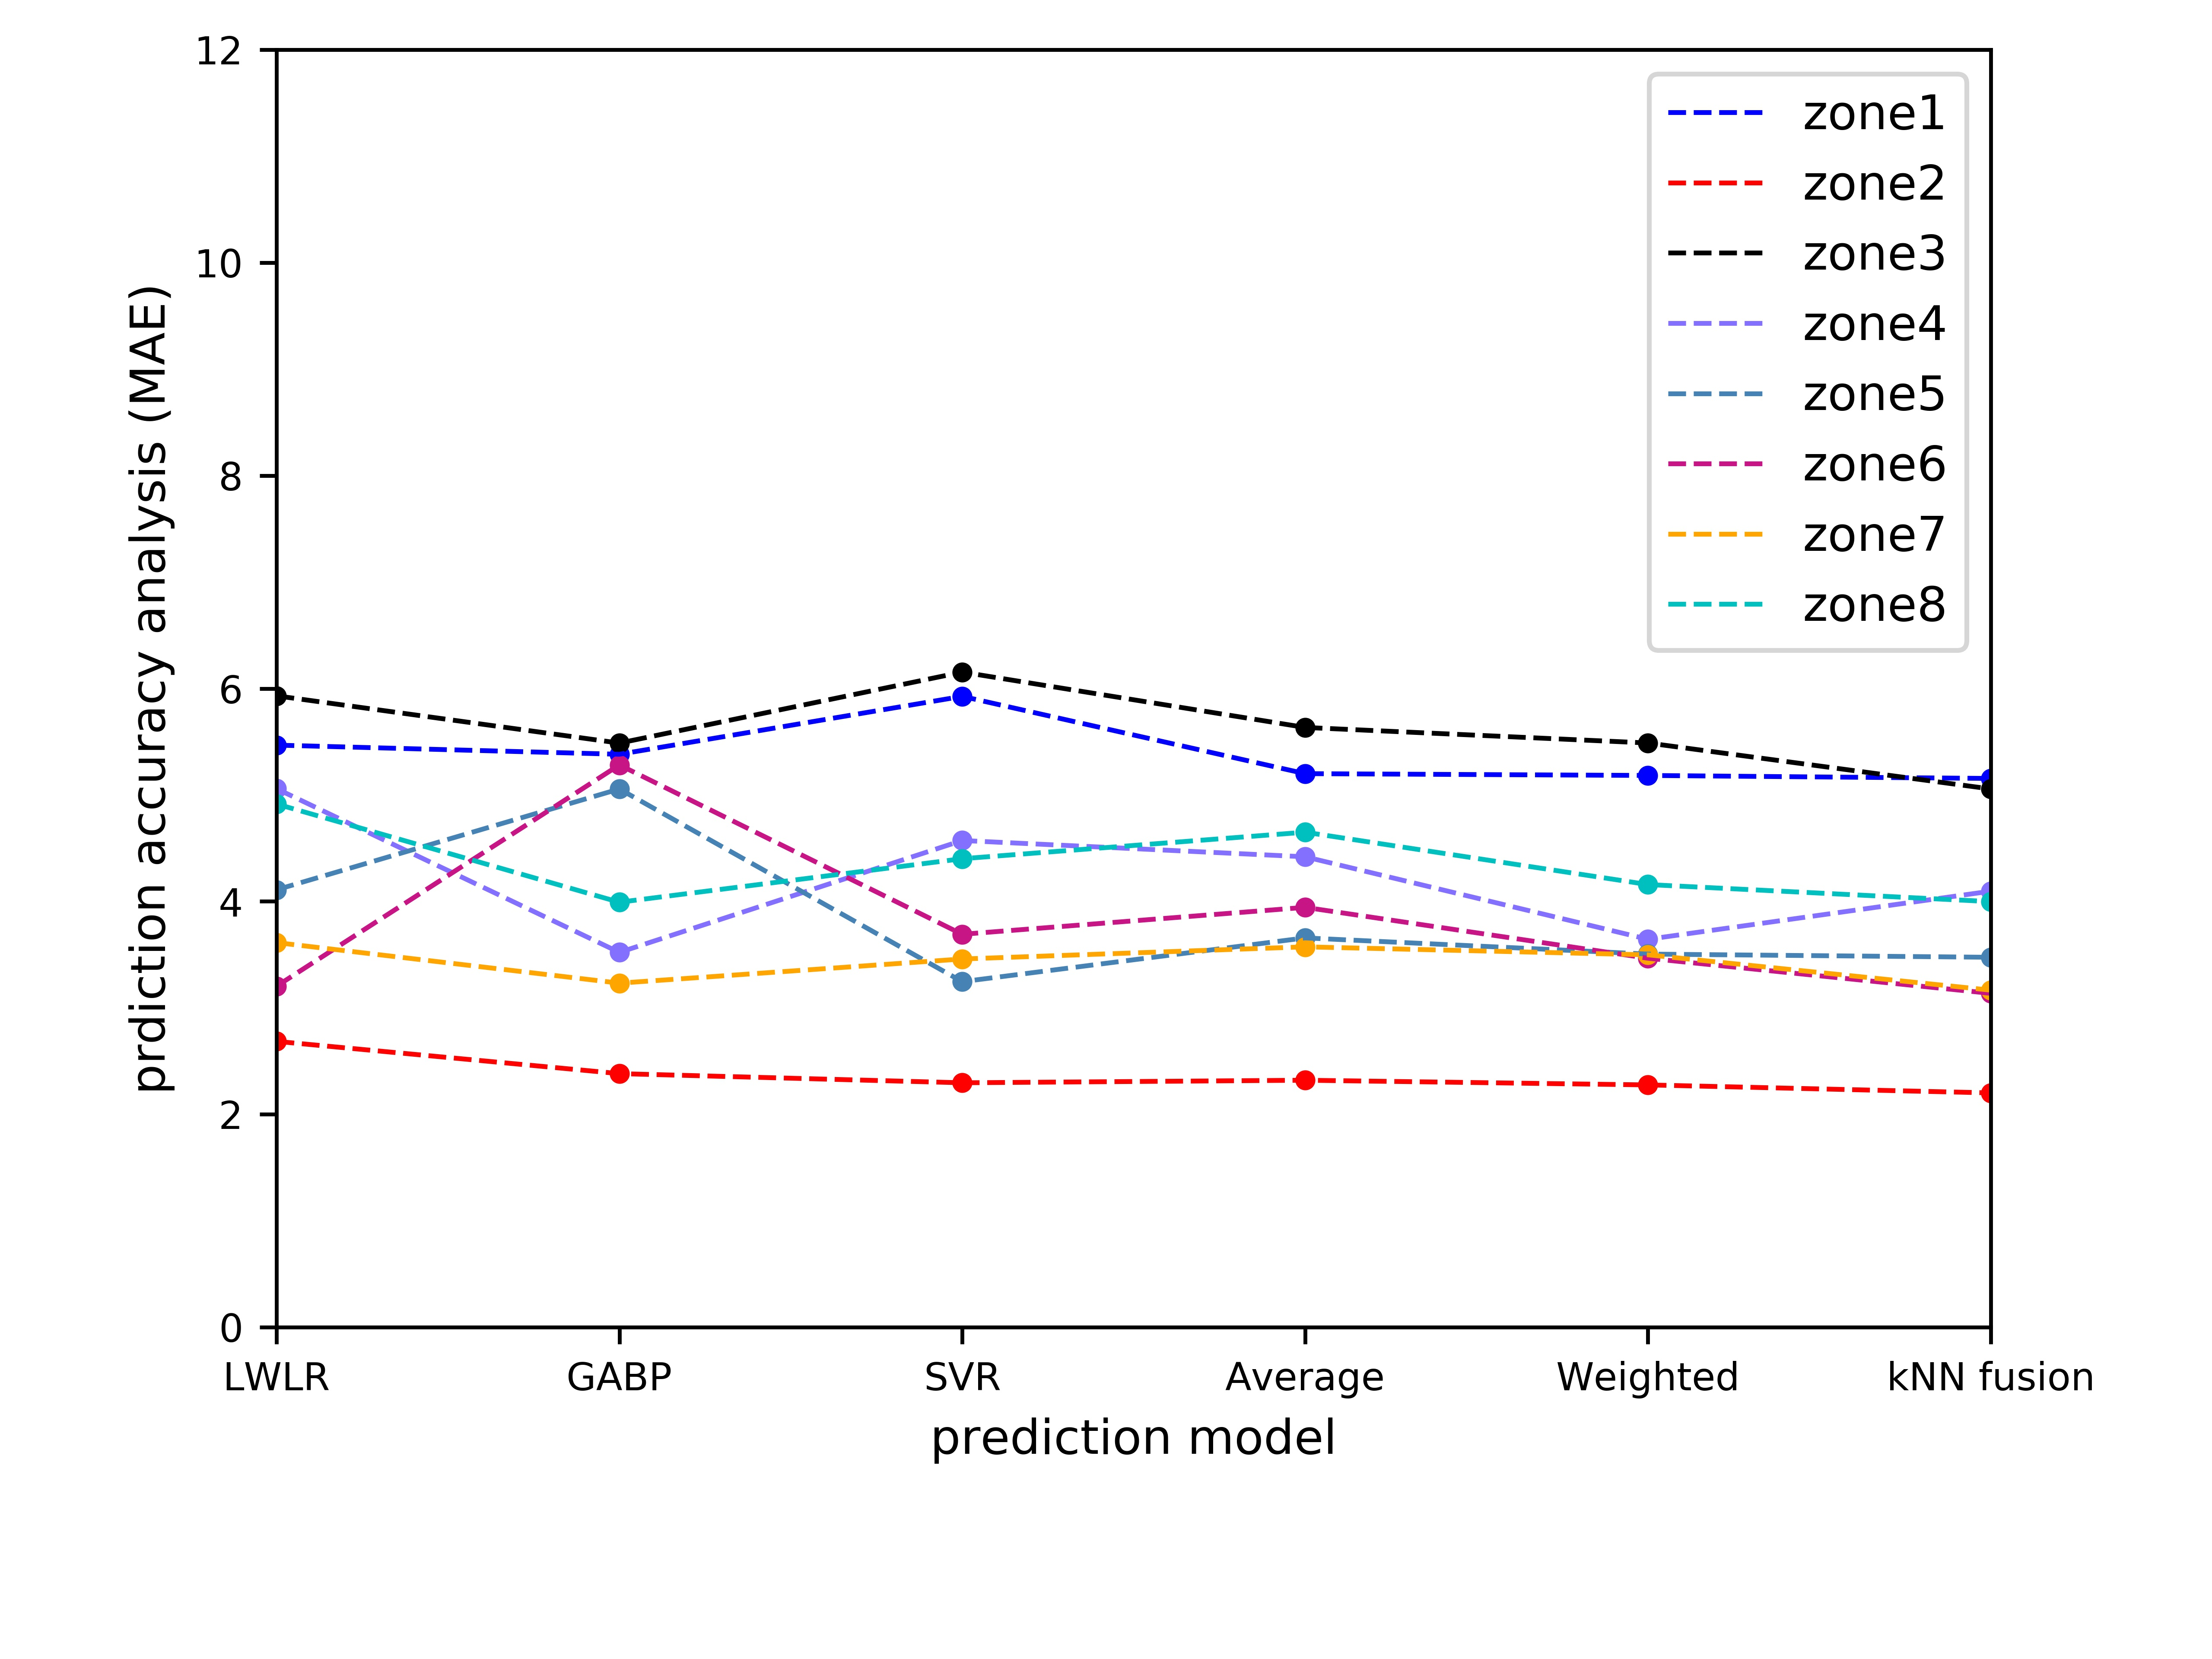
\includegraphics[width=.8\linewidth]{MAE}  
    \caption{MAE analysis}
    \label{fig:sub-first}
  \end{subfigure}\hfil
  \begin{subfigure}{.5\textwidth}
    \centering
    % include second image
    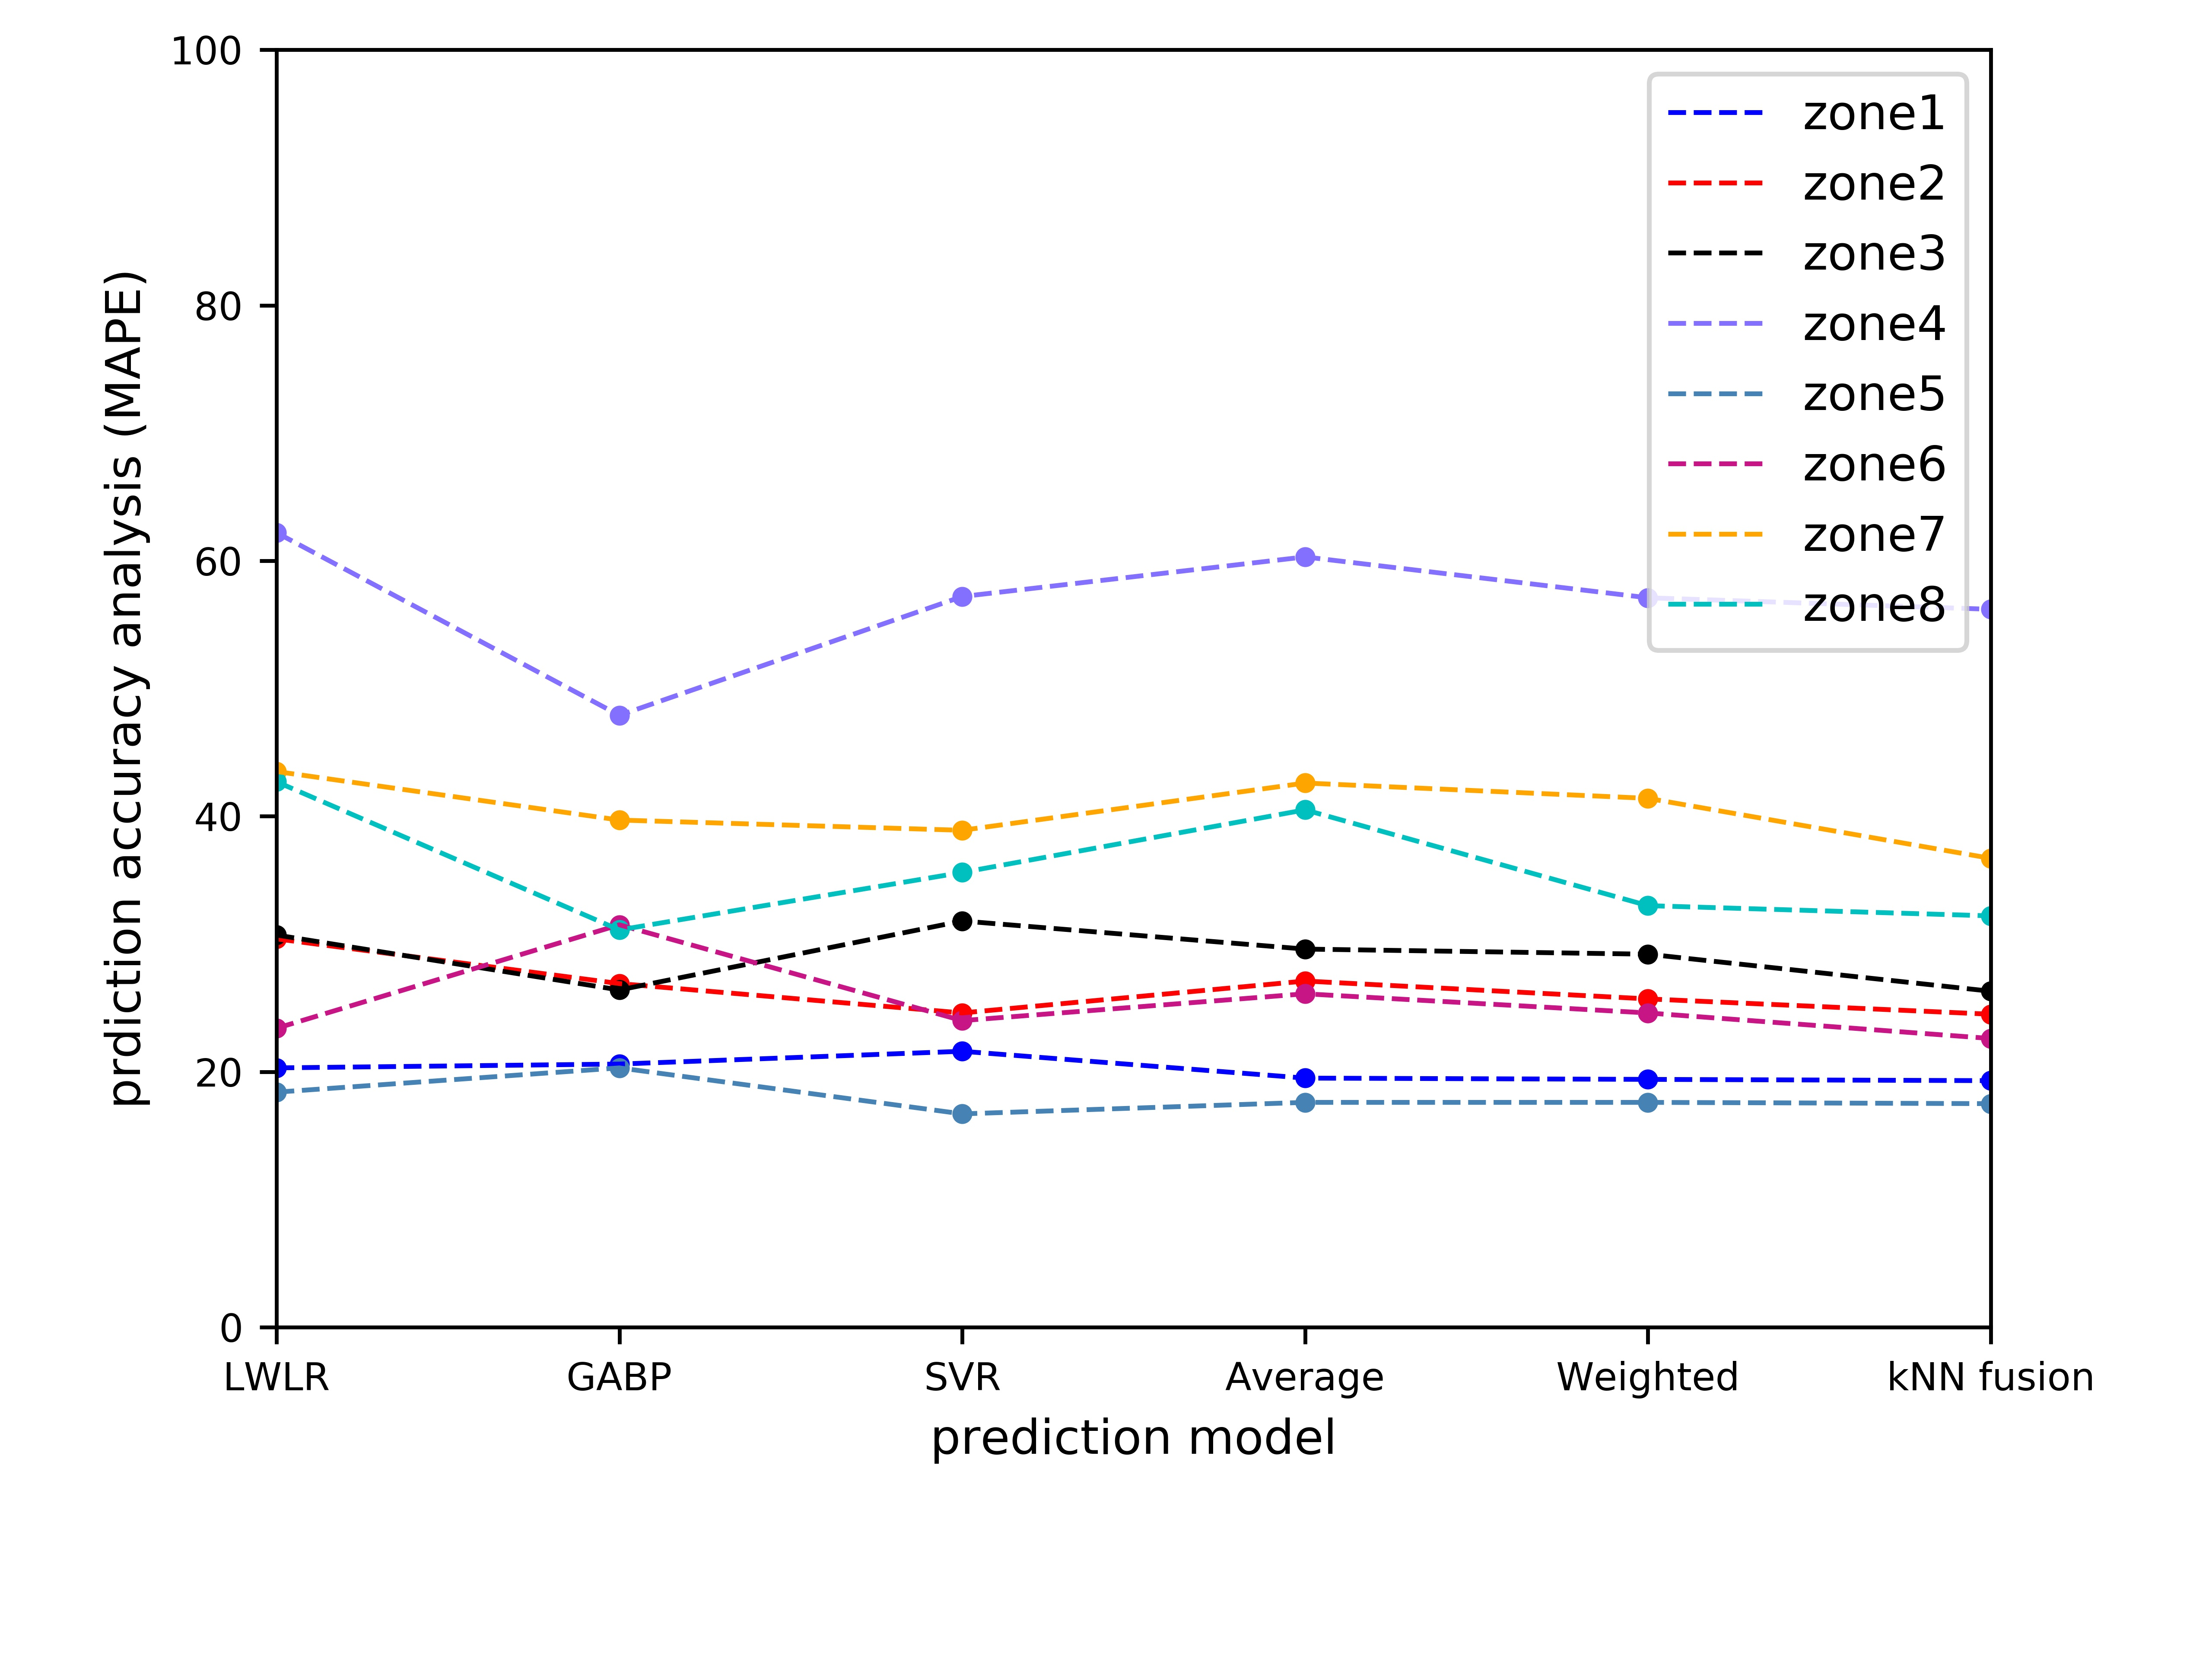
\includegraphics[width=.8\linewidth]{MAPE}  
    \caption{MAPE analysis}
    \label{fig:sub-second}
  \end{subfigure}

  \medskip
  \begin{subfigure}{.5\textwidth}
    \centering
    % include third image
    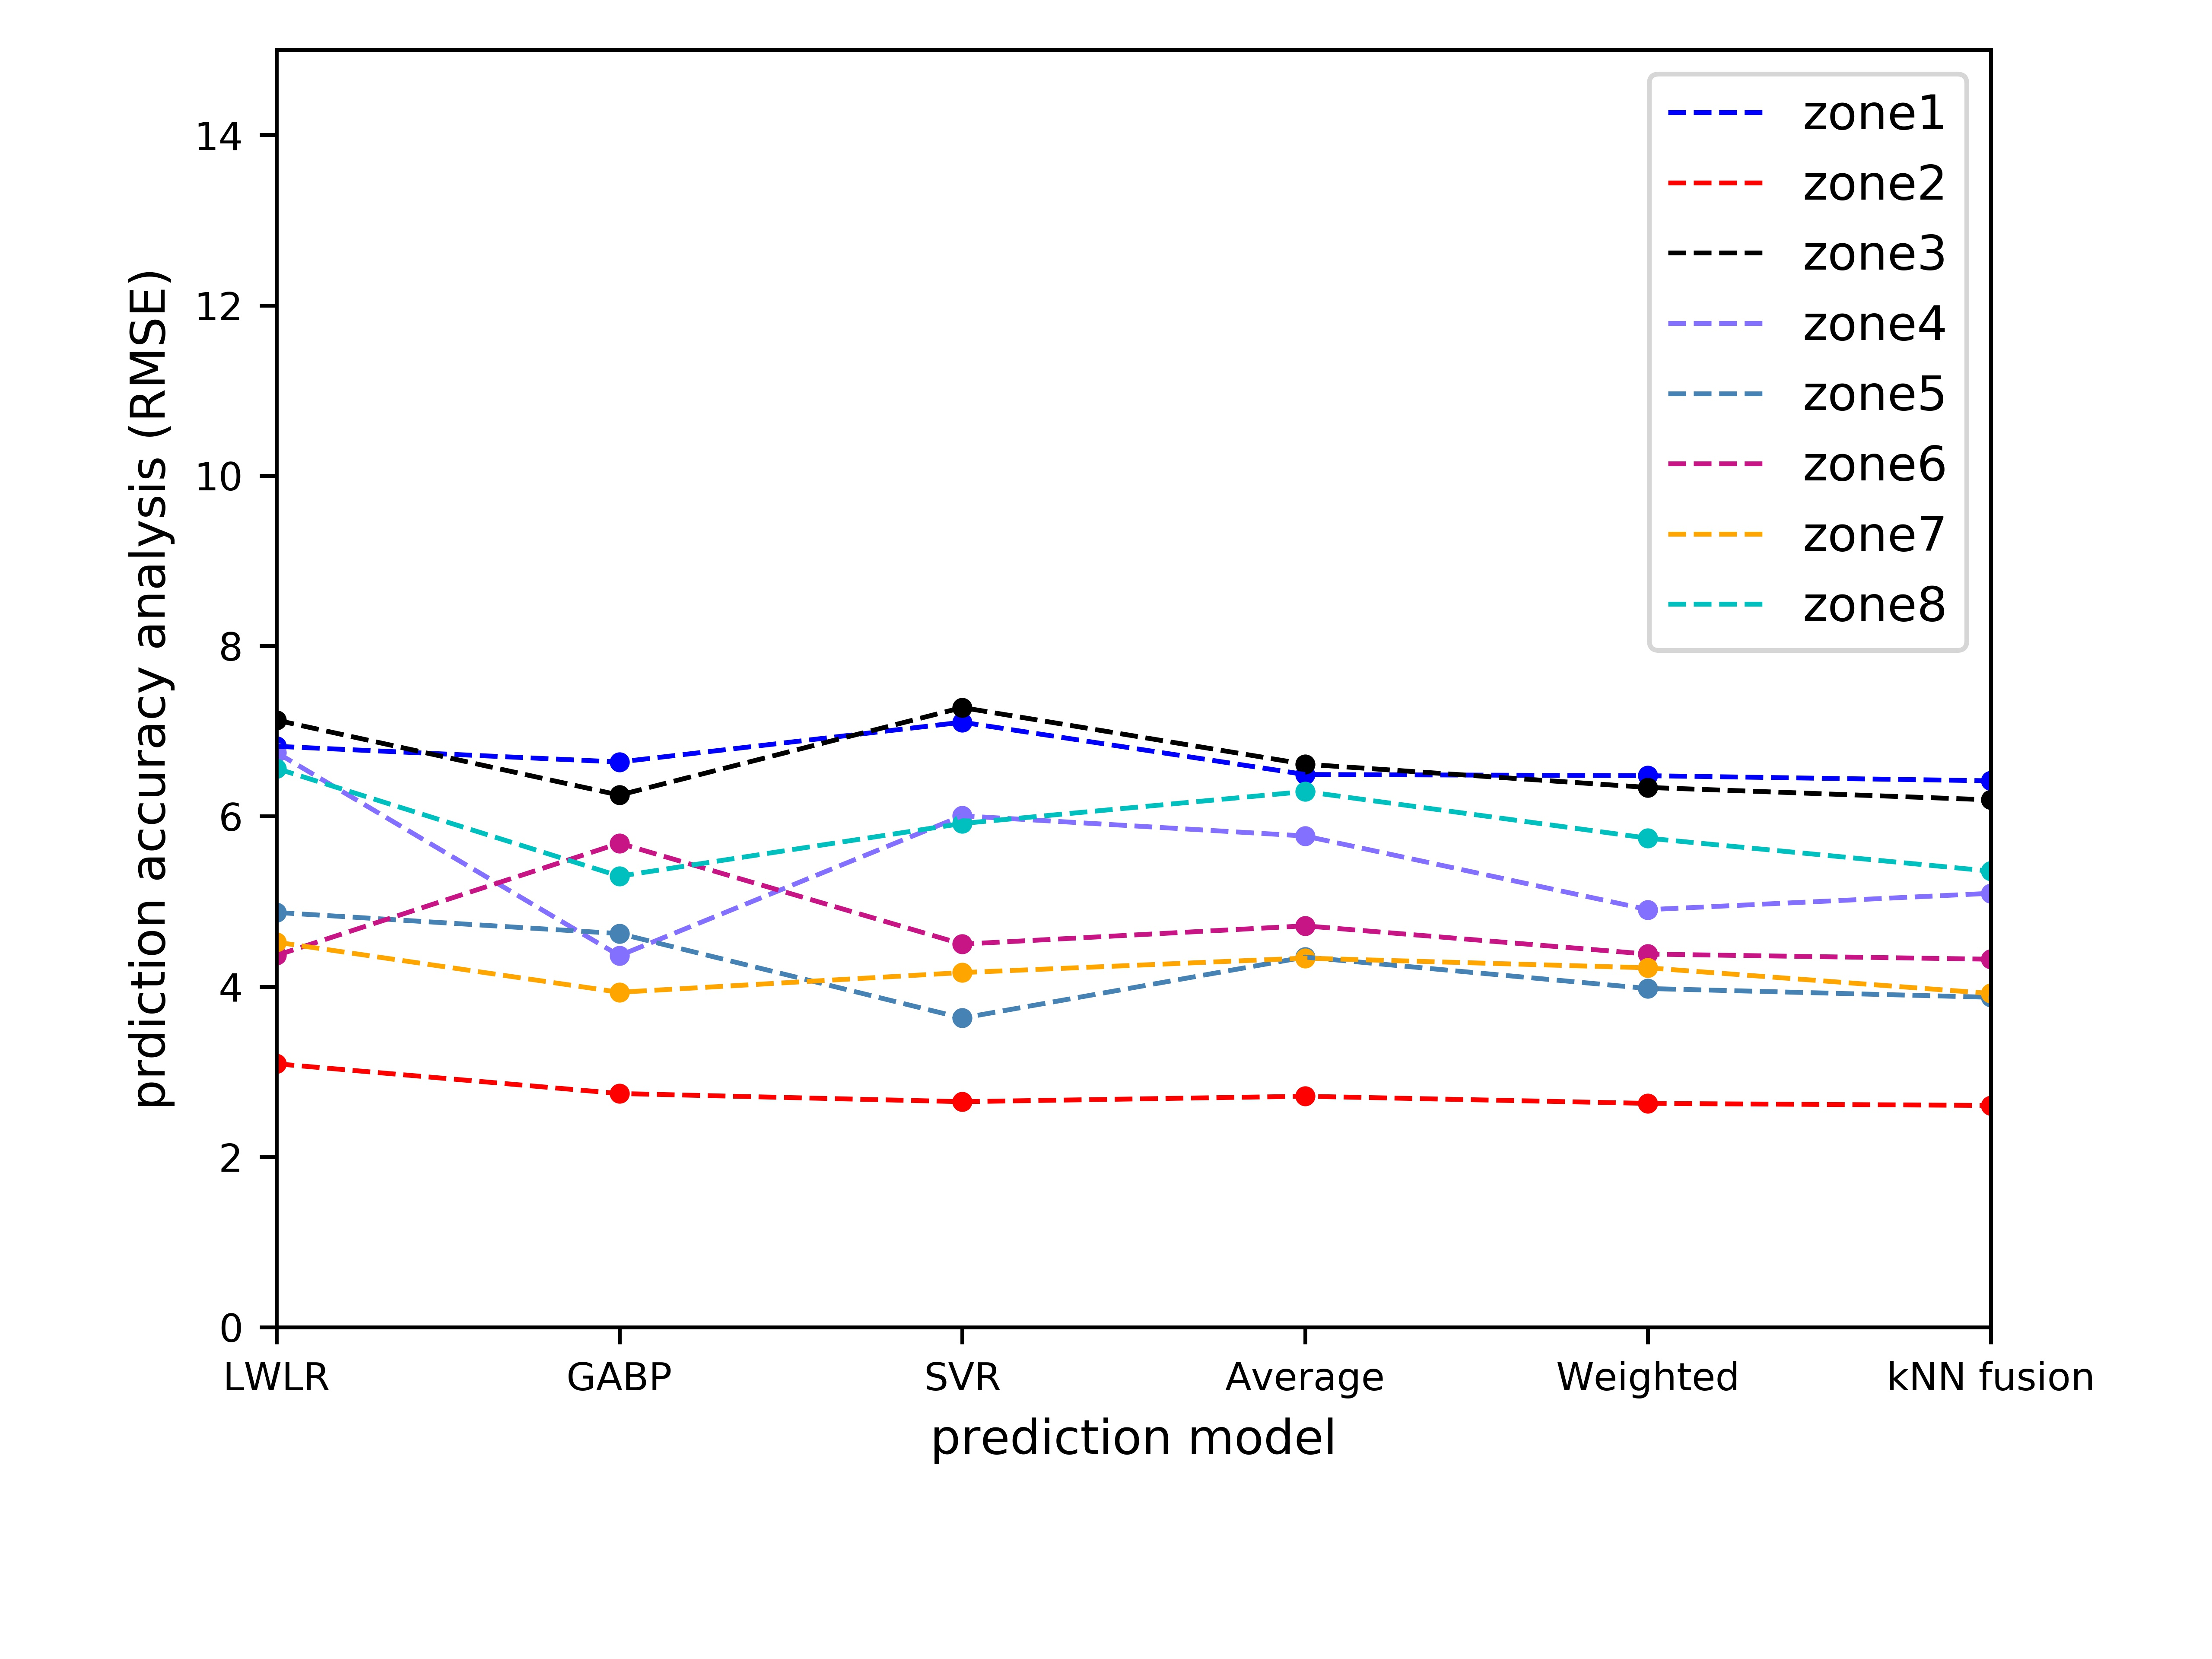
\includegraphics[width=.8\linewidth]{RMSE}  
    \caption{RMSE analysis}
    \label{fig:sub-third}
  \end{subfigure}\hfil
  \begin{subfigure}{.5\textwidth}
    \centering
    % include fourth image
    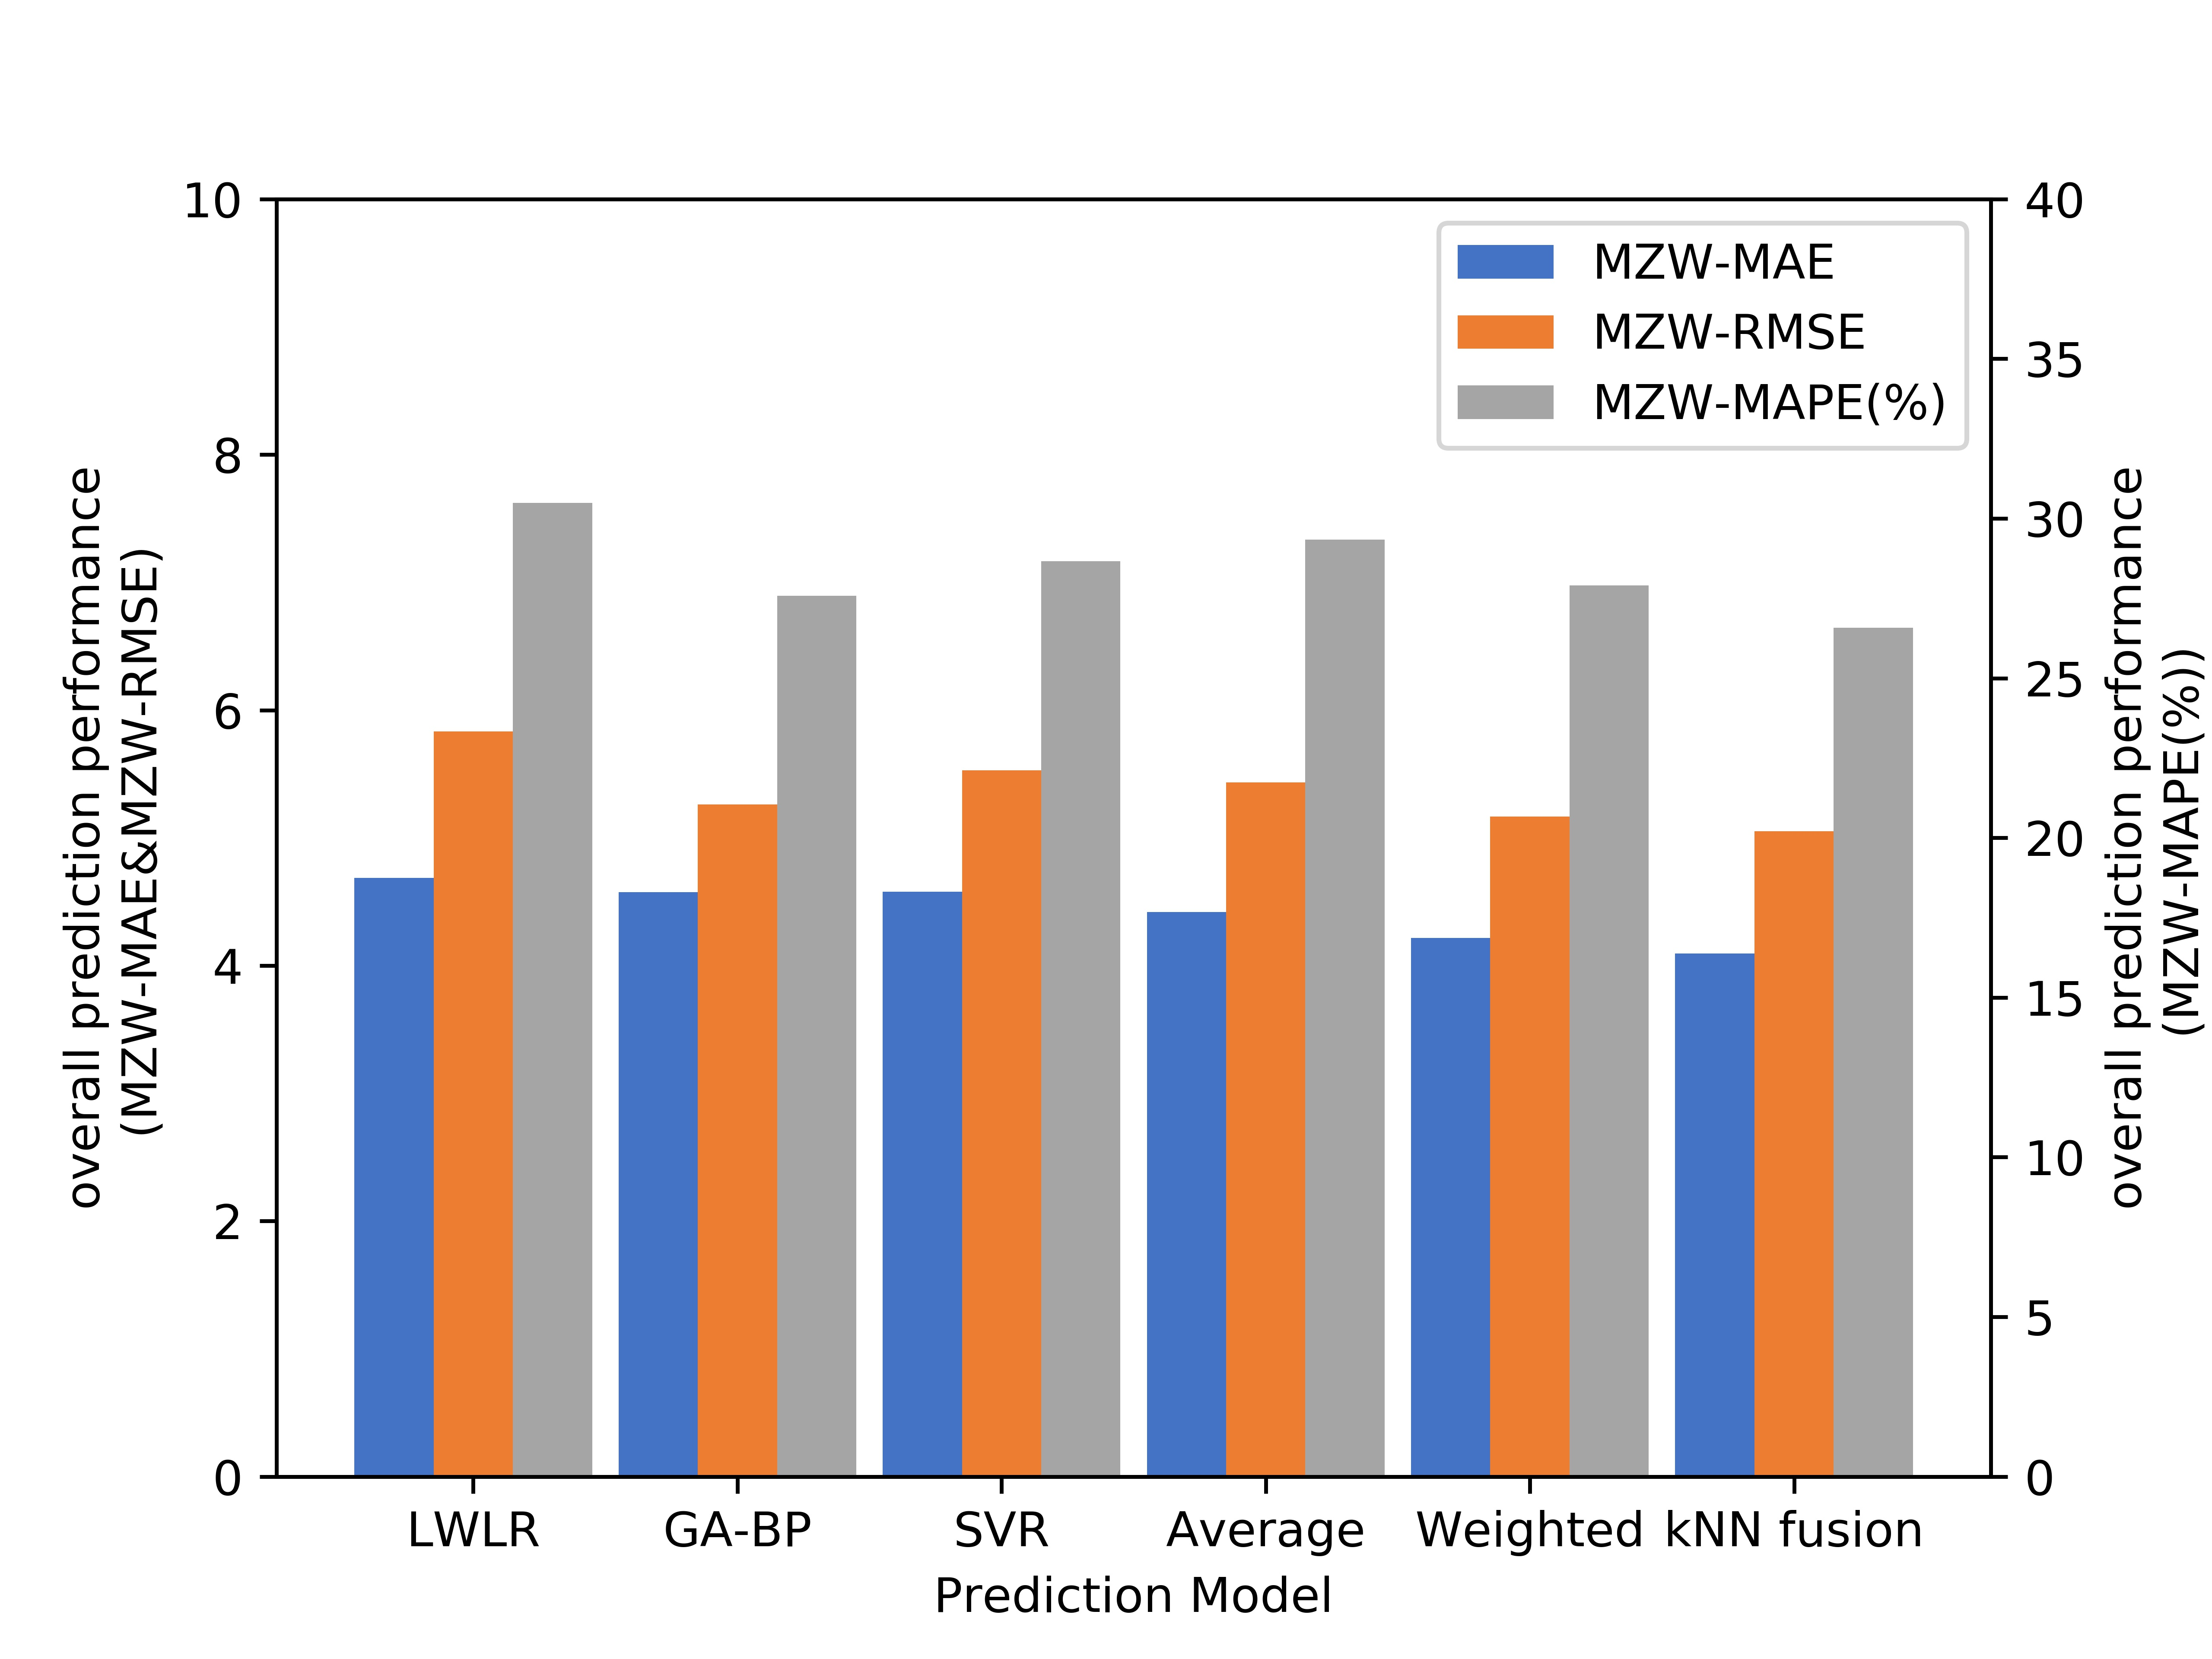
\includegraphics[width=.8\linewidth]{all}  
    \caption{Overall prediction performance}
    \label{fig:sub-fourth}
  \end{subfigure}
  \caption{Prediction accuracy analysis}
  \end{figure*}
In Zone 1, the values of MAPE using average and weighted fusion based methods are 19.5\% and 19.4\%, while the value of the MAPE using kNN fusion based method is 19.3\%. Meanwhile, compared with average and weighted fusion based method, the value of MAE and RMSE using kNN fusion based method are relatively lower than other prediction models, which are 5.155 and 6.416 respectively. In the same way, kNN fusion based method gives the most accurate results than other prediction models in Zone 2 (e.g. 2.604 orders/h of RMSE), Zone 3 (e.g. 6.192 orders/h of RMSE), Zone 6 (e.g. 4.321 orders/h of RMSE), Zone 7 (e.g. 3.919 orders/h of RMSE). 

In Zone 4 and Zone 8, GABP is better. But the performance of the kNN fusion based method is also significantly better than other prediction models in Zone 4. Compared with MAPE of average fusion based method, the improvement of kNN fusion based method is 4\%. Besides, the performance of the  fusion based method is second only to that of GABP in Zone 8, 3.998 orders/h of MAE, 32.2\% of MAPE, 5.355 orders/h of RMSE. By contrast, in Zone 5, the best performing prediction model is SVR, but the second is kNN fusion based method, the performance of kNN fusion based method is only 0.8\% difference from that of SVR in terms of MAPE.

In terms of overall prediction performance analysis, the values of MZW-MAE, MZW-MAPE, MZW-RMSE of kNN fusion based method are lowest in these six prediction methods, which are 4.095 orders/h, 26.579\% and 5.05 orders/h respectively and this indicates that kNN fusion based method could give a better prediction result in multi-zone prediction.

From the viewpoint of fusion methods, simple fusion method including average fusion based method and weighted fusion method only provide moderate improvements to the overall prediction accuracy, but kNN fusion based method can have a better prediction performance in this case of predicting short-term order demand. For example, in Zone 7, the MAPE value is reduced to 36.7\% from 38.9\% which is the best result using the individual prediction model, in contrast with 42.6\% in average fusion based method and 41.4\% in weighted fusion based method.

\section{Conclusion}
In order to help facilitate city-scale travel operation management in megacity,
this project proposes a multi-zone order demand prediction model to divide order
zones through K-Means++ spatial clustering algorithm, and predict order demand
in different divided zones based on six different prediction models, including
kNN fusion based method, LWLR, GA-BP Neural Network, SVR, average fusion based
method and weighted fusion based method. This study takes taxi order demand to
Shenzhen International Airport as a case study to divide the order area and predict
the order demand in different zones. The result indicates that it is effective
to use multi-zone travel demand prediction model to divide the order zones and
predict order demands. According to the systematic comparison analysis, GA-BP
Neural Network, SVR and kNN fusion based method have relatively good predictive
performance in individual zones based on three prediction accuracy indicators (MAE, MAPE, RMSE). 
However, according to multi zone weighted indicators, MZW-MAE, MZW-MAPE and MZW-RMSE,
the overall prediction performance of kNN fusion based method for multi-zone order demand is the best.
Overall, we can support that in the case of city-scale order prediction,
using multi-zone prediction model with kNN fusion based method can be effective.
And it could be suggested, the multi-zone prediction model with kNN fusion based method
proposed in this study can be served as a basis of scheduling optimization at city-scale.
However, limited by data availability, our case study is special, and in the future work,
we would use data from more scenarios for verification, and then get more comprehensive
conclusion.


\section{Contributions}
We are three member team, Chenyu worked on the data
extraction part, prepared all the features with necessary
plots; Pengshun worked on the algorithm implementation with the sklearn framework;
Chenxi worked on the overall methodology
design on the benchmark on this task and paper
write up. All the members joined in the results analysis
and future work discussion and write-up collaborations.

%%
%% The next two lines define the bibliography style to be used, and
%% the bibliography file.
\bibliographystyle{ACM-Reference-Format}
\bibliography{sample-ref}

\end{document}
\endinput
%%
%% End of file `sample-workshop.tex'.
